\subsection{Trigonometrie \texorpdfstring{ \hfill S.97-99}{S.97-99}}
\vspace{2pt}
        %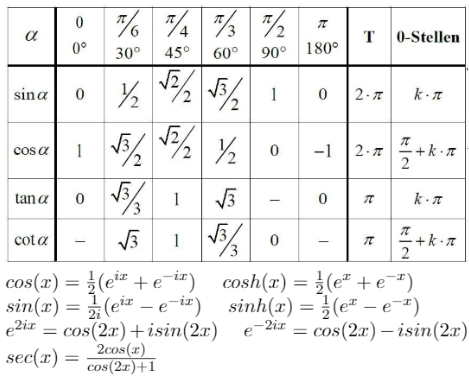
\includegraphics[width= \linewidth]{src/Appendix/Standardwerte_Trigonometrie.png}
\renewcommand{\arraystretch}{2}
$
\begin{array}{|l||c|c|c|c|c|c||c|c|}
    \hline
    \textrm{rad} & 0 & \frac{\pi}{6} & \frac{\pi}{4} & \frac{\pi}{3} & \frac{\pi}{2} & \pi & \textrm{\textbf{T}} & \textrm{\textbf{Nst.}}  \\
    \grad & 0^o & 30^o & 45^o & 60^o & 90^o & 180^o & &  \\
    \hline 
    \sin\alpha & 0 & \frac{1}{2} & \frac{\sqrt{2}}{2} & \frac{\sqrt{3}}{2} & 1 & 0 & 2\pi & k\!\cdot\!\pi \\
    \hline 
    \cos{\alpha} & 1 & \frac{\sqrt{3}}{2} & \frac{\sqrt{2}}{2} & \frac{1}{2} & 0 & -1 & 2\pi & \frac{\pi}{2}\!+\!k\!\cdot \!\pi \\
    \hline 
    \tan \alpha & 0 & \frac{\sqrt{3}}{3} & 1 & \sqrt{3} & - & 0 & \pi & k\!\cdot \! \pi \\
    \hline 
    \cot \alpha & - & \sqrt{3} & 1 & \frac{\sqrt{3}}{3} & 0 & - & \pi & \frac{\pi}{2}\!+\!k\!\cdot \!\pi \\
    \hline 
\end{array}
$

\begin{align*}
    \cos x &= \frac{1}{2}(e^{ix} + e^{-ix}) & \cosh x &= \frac{1}{2}(e^x + e^{-x}) \\
    \sin x &= \frac{1}{2i}(e^{ix} - e^{-ix}) & \sinh x &= \frac{1}{2}(e^x - e^{-x} \\
    e^{2ix} &= \cos(2x)\!+\! i\sin(2x) & e^{-2i} &= \cos(2x)\!-\!i\sin(2x) \\
    \sec x &= \frac{2 \cos x}{\cos(2x) + 1} && \\ 
\end{align*}

%\subsection{Koordinatentransformation}
%        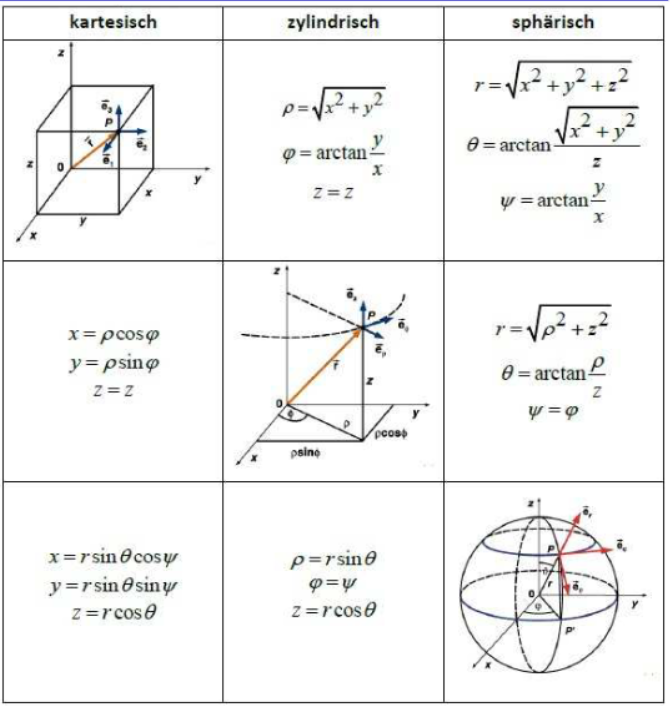
\includegraphics[width = \linewidth]{src/Appendix/Koordinatentransformation.png}
%        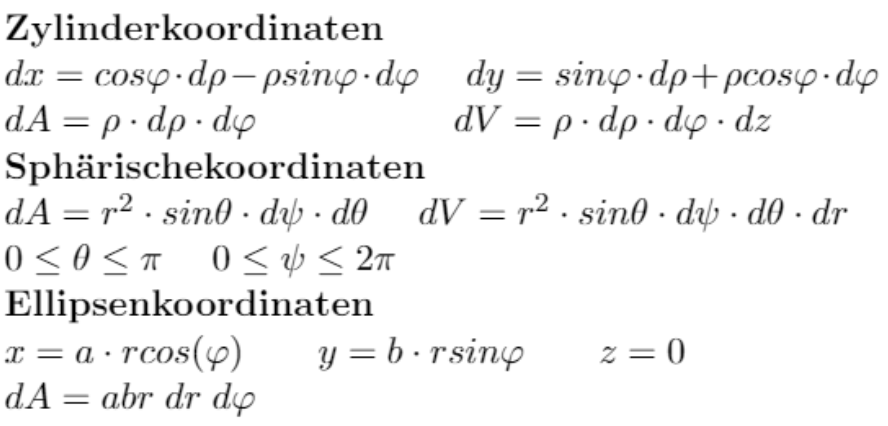
\includegraphics[width = \linewidth]{src/Appendix/Formel Koordinatentransformation.png}
% !TeX root = ../../ZF_bmicha_Ana.tex
\subsection{Cosinus und Sinus - Integrale \texorpdfstring{\hfill S.74}{S.74}}
    
    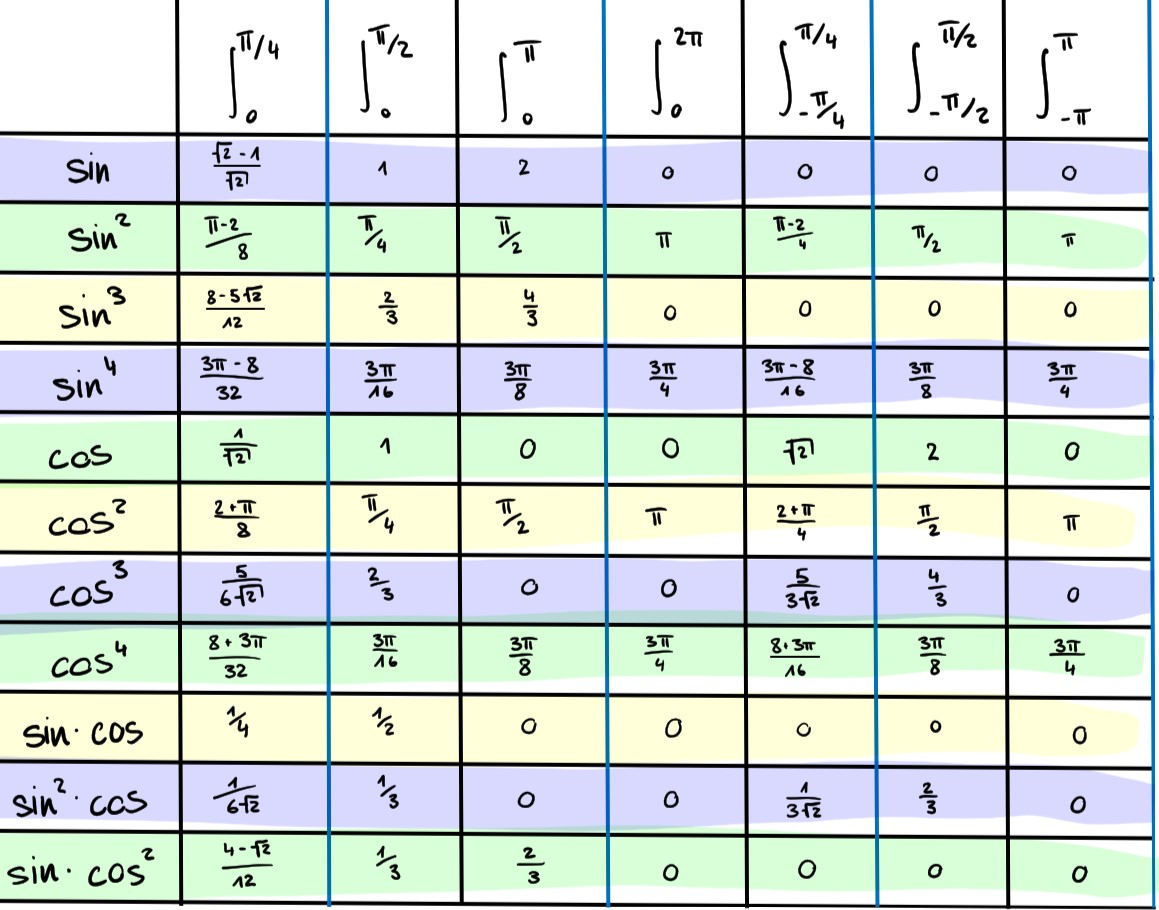
\includegraphics[width = \linewidth]{src/Appendix/integraltabelle_sin_cos.jpg}
    Für $a,b \in \mathbb{N}$ und $n \geq 2$, gelten:
    \begin{align*}
        \int_{a \cdot \frac{\pi}{2}}^{b \cdot \frac{\pi}{2}} \sin^n(x) \ dx 
            &= \frac{n-1}{n} \int_{a \cdot \frac{\pi}{2}}^{b \cdot \frac{\pi}{2}} \sin^{n-2}(x) \ dx\\[0.5em]
        \int_{a \cdot \frac{\pi}{2}}^{b \cdot \frac{\pi}{2}} \cos^n(x) \ dx 
            &= \frac{n-1}{n} \int_{a \cdot \frac{\pi}{2}}^{b \cdot \frac{\pi}{2}} \cos^{n-2}(x) \ dx
    \end{align*}

\subsection{Ableitungsregeln \texorpdfstring{\hfill S.62-65}{S.62-65}}
        
        Kettenregel 
       $$[f(x) \cdot  g(x)]' = f'(x)\cdot g(x) + f(x) \cdot  g'(x)$$
       Quotientenregel
       $$ [\frac{f(x)}{g(x)}]' = \frac{f'(x)\cdot g(x) - f(x)\cdot g'(x)}{g^2(x)} $$
       Verallgemeinerte Kettenregel
       $$F'(x(t), y(t)) = f_x (x(t), y(t)) \cdot  \dot{x} + f_y (x(t), y(t)) \cdot  \dot{y} $$
       
\subsection{Additionstheoreme \texorpdfstring{\hfill S.99}{S.99}}
    \textbf{$\textrm{cot} = \textrm{tan}^{-1}$}
    \begin{align*}
            1 + cot^2(x) = \frac{1}{sin^2(x)} && cot(a \pm b) = \frac{cot(a)cot(b) \mp 1}{cot(a) \pm cot(b)} \\
            cot(2a) = \frac{cot^2(a) -1}{2 cot(a)}
    \end{align*}
    \textbf{a/2}
    $$ sin \left( \frac{a}{2} \right) = \pm \sqrt{\frac{1}{2}\cdot (1-cos(a)} $$
    $$ cos \left( \frac{a}{2} \right) = \pm \sqrt{\frac{1}{2}\cdot (1+cos(a)} $$

\subsection{Integrationsregeln \texorpdfstring{\hfill S.70-72}{S.70-72}}
       $$ \frac{d}{dx} \int_a^{u(x)} f(u) du = f(g(x)) * g'(x)$$
       Partielle Integration: 
       $$ \int u'\cdot v dx = u\cdot v - \int u\cdot v' dx $$
       Substitution 1. Art \vspace{2pt}
       \begin{center}
           $ \int_a^b f(u(x))u'(x) dx = \int_{u(a)}^{u(b)} f(z) dz $, wobei $ z = u(x)$
       \end{center}
       
       Substitution 2. Art \vspace{2pt}
       \begin{center}
           $ \int_a^b f(x) dx = \int_{u(a)}^{(u(b)} f(u(z))\cdot u'(z) dz $, wobei $ x = u(z)$
       \end{center}

\subsection{Partialbruchzerlegung, Polynomfkt. \texorpdfstring{\hfill S.21+57}{S.21+57}}
        \vspace{3pt}
       \begin{enumerate}
           \item einfache Nullstelle: $ \frac{A}{x - x_0}$
           \item doppelte Nullstelle: $\frac{A}{x - x_0} + \frac{B}{(x-x_0)^2} $
           \item komplexe Nullstelle: $ \frac{A*x + B}{(z.B.: x^2 + 1)}$
       \end{enumerate}

\subsection{Komplexe Zahlen \texorpdfstring{\hfill S.18-19}{S.18-19}}
       \vspace{3pt}
       
       \def\arraystretch{1.5}
       \begin{tabular*}{\linewidth}{ll}
           imaginäre Einheit: & $i^2 = 1$ \\
           Normalform: & $ z = a + ib $ \\
           Polarform: & $ z = r(cos\phi + isin\phi) $ \\
           Exponentialform: & $ z = re^{i\phi} $ \\
           Konjugierte: & $ \bar{z} = a\!-\!ib = r(cos\phi\!-\!isin\phi) = re^{-i\phi} $
       \end{tabular*}
       \vspace{5pt}
       
       Winkel grösser als $2\pi$ können auf ihr Äquivalent im Bereich $[0; 2\pi]$ reduziert werden \\[3pt]
       Form: $\arg (z) = \phi = \textrm{Winkel}$ \vspace{6pt}
       
       \textbf{Umrechnungsformeln:}
       
       \vspace{3pt}
       
       \begin{tabular*}{\linewidth}{ll}
           Normal- $\rightarrow$ Polarform: & $ r = \sqrt{a^2 + b^2} $ \\
           & $ cos\phi = \frac{a}{r}, sin\phi = \frac{b}{r} $ \\
           Polar- $\rightarrow$ Normalform: & $ a = rcos\phi, b = rsin\phi $
       \end{tabular*}
       
       \vspace{5pt}
       
       \textbf{Operationen siehe S.18}\\[3pt]
       \textit{Hinweis: bei Multiplikation einer kompl. Zahl mit Betrag 1 dann wird um den Ursprung rotiert.} \vspace{5pt}
       
       \cbreak
       
       \textbf{Potenzieren:}
       
       $$z^n = r^n e^{in\phi} $$
       
       \textbf{Wurzel ziehen:}
       
       Sucht man $n$ Wurzeln $w$ der komplexen Zahlen $z$, so setzt man $k = 0, 1,..,n-1$ in die folgende Fomrel ein: 
       $$ w_k = \sqrt[k]{|z|} \cdot e^{i(\frac{\phi}{k} + \frac{2\pi k}{k})} $$

       \begin{minipage}{0.49\linewidth}
           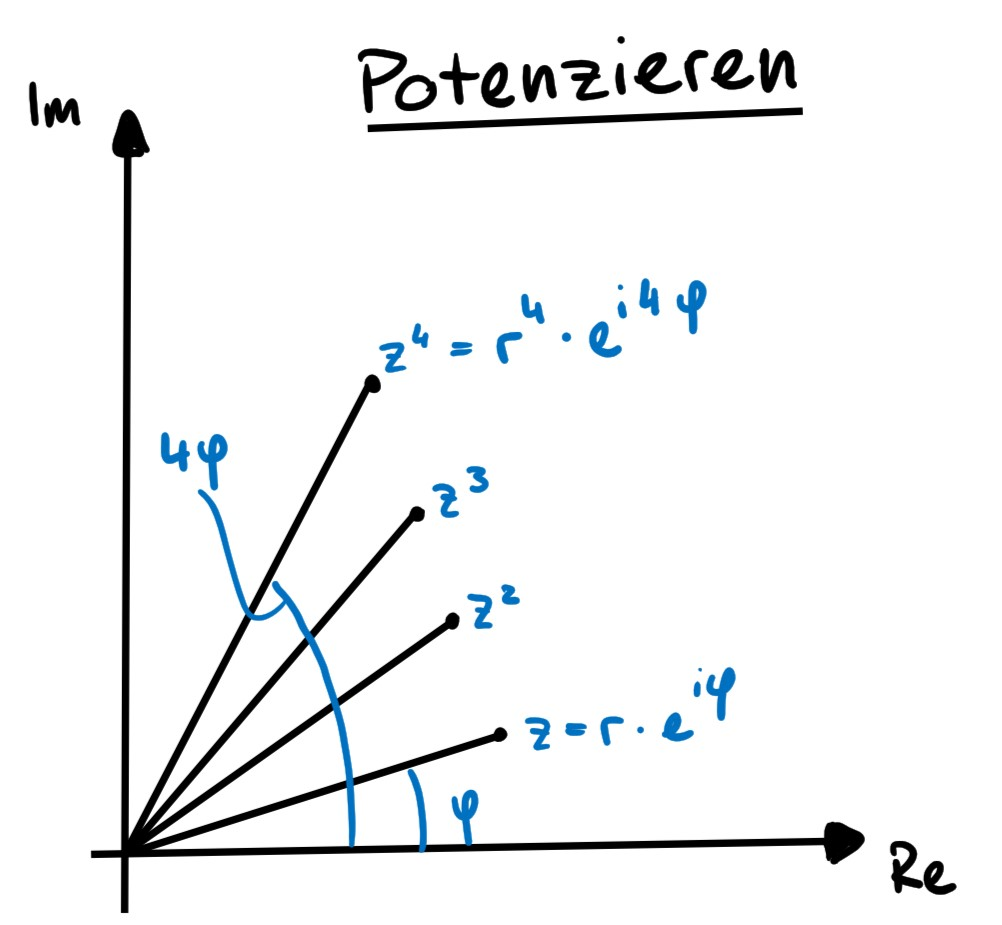
\includegraphics[width=\linewidth]{src/Appendix/1_komplexe_Zahlen_potenzieren.jpg}
       \end{minipage}
       \begin{minipage}{0.5\linewidth}
        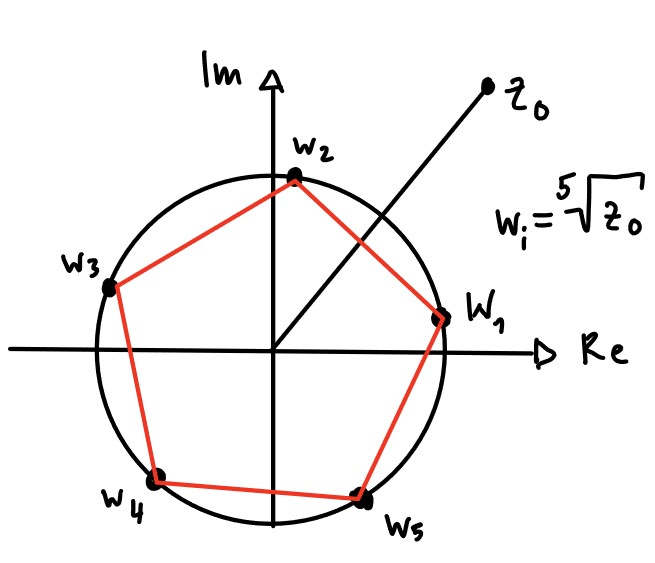
\includegraphics[width= \linewidth]{src/Appendix/kompl_Zahlen_wurzeln.jpg}
       \end{minipage}